\newcommand{\radac}{RAdAC\ }
\myChapter{Access Control e Usage Control}
\label{cap:accessControl}
Al giorno d’oggi esistono moltissimi sistemi capaci di condividere dati e
risorse computazionali, ed impedire accessi non autorizzati è diventata
una priorità inderogabile. Ad esempio, molti dati personali possono essere
raccolti durante alcune attività quotidiane, dunque diventa necessario
proteggere questi dati da malintenzionati. Questa è solo una delle tante
ragioni per cui esistono sistemi di \textit{Access Control}, ovvero dei sistemi
definiti da un insieme di condizioni che permettono di creare una prima
linea difensiva contro accessi indesiderati.

\section{Storia dell'Access Control}
\label{sec:history}



Negli anni sono stati proposti diversi approcci per cercare di definire un
modello efficiente e scalabile. Andremo ora ad eseguire una classificazione
dei modelli di Access Control, seguendo la catalogazione del NIST \cite{NISTACM}.
Il primo di questi si chiama
\textit{Access Control Lists} (ACLs) ed è stato proposto intorno al 1970 spinto
dall’avvento dei primi sistemi multi utente.\par
Successivamente è nato un nuovo modello chiamato Role-based \textit{Access
Control (RBAC)} che modifica alcuni aspetti di ACL in modo da rimuovere
molte delle limitazioni di quest’ultimo.\par
Uno dei problemi di RBAC è l’impossibilità di differenziare membri
di uno stesso gruppo in modo da negare o permettere accessi sulla base
di singoli attributi, ed è per venire in contro a questa necessità che è
stato implementato un nuovo modello chiamato \textit{Attribute Based Access
Control (ABAC)}, dove le decisioni vengono prese in base ad un set di
attributi legati al richiedente, all’ambiente ed alla risorsa per cui si chiede
l’accesso.\par
Anche questo modello però ha delle limitazioni che vengono fuori
quando il numero di risorse da gestire è elevato, motivo per cui nasce
\textit{Policy-based Access Control (PBAC)}. PBAC migliora e standardizza il
modello ABAC combinando attributi dalle risorse, dall’ambiente e dal
richiedente con informazioni di un particolare insieme di circostanze
sotto le quali la richiesta è stata effettuata.\par
Ciononostante, le organizzazioni non sono statiche, ma in continua evoluzione, e devono rispondere
ad una varietà di stimoli, che possono essere legali, economici, finanziari,
di mercato o altri fattori di rischio. Anche tecniche avanzate,
come per esempio ABAC e PBAC, non riescono in maniera sufficiente a
rispondere ai bisogni di dinamismo e cambiamenti dei livelli di rischio,
motivo per cui è nato Risk-adaptive Access Control (RAdAC ) che fornisce
un modello adattabile al settore enterprise.


\subsection*{Access Control Lists (ACLs)}
\label{sub:ACL}

ACL è il più datato e basico modello di controllo agli accessi. Prende piede intorno agli anni 70
grazie all'avvento dei sistemi multi utente i quali necessitano di limitare l'accesso a file e dati condivisi, infatti i primi sistemi ad utilizzare questo modello sono stati sistemi di tipo UNIX. \par
Con la comparsa della multiutenza per sistemi ad uso personale lo standard ACL è stato implementato in molte più ambienti come sistemi UNIX-Like e Windows. \par
Nonostante negli anni sono stati sviluppati modelli più complessi ACL viene comunque usato nei sistemi operativi recenti, come si può vedere in figura \ref{fig:acl_osx} OS X sfrutta questo standard per la gestione dei permessi sul filesystem.
Il concetto dietro ACL è uno dei più semplici, in quanto ogni risorsa del sistema che deve essere controllata ha una sua lista che ad ogni soggetto associa le azioni che può effettuare sulla risorsa ed il sistema operativo, quando viene fatta richiesta decide in base alla lista se dare il permesso o meno. \\ \par
Per esempio, sempre in figura \ref{fig:acl_osx}, si può vedere come \textit{test\_folder} sia la risorsa da controllare, \textit{federicoschipani}, \textit{staff} e \textit{everyone} siano i soggetti e le azioni associate sono, in questo caso, \textit{Read \& Write} al primo soggetto e \textit{Read only} agli altri due.
\MyFigure{acl_osx}{ACL in OS X}{1}
La semplicità di questo modello non richiede grandi infrastrutture sottostanti, infatti implementarlo dal punto di vista applicativo risulta abbastanza semplice attraverso l'uso di linguaggi ad alto livello come Python o Java, poiché le strutture che servono per implementare questo standard sono già definite. \par
Questo elevato grado di relativa facilità di implementazione però ha anche un aspetto negativo che si manifesta quando si ha a che fare con grandi quantità di risorse. Ogni volta che viene richiesto l'accesso ad una risorsa da parte di un entità, utente o applicazione che sia, è necessario verificare nella lista associata, il che lo rende abbastanza oneroso dal punto di vista computazionale.\\ \par
Un altro lato negativo emerge quando bisogna effettuare modifiche ai permessi di una determinata risorsa, in quanto è necessario andare ad operare sulla lista di quest'ultima, il che rende questo compito incline ad errori ed oneroso dal punto di vista del tempo.


\subsection*{Role-based Access Control (RBAC)} % (fold)
\label{sub:role_based_access_control}

RBAC è un po' l'evoluzione di ACL, in quanto tende a correggerne alcuni, se così si possono chiamare, difetti. \par
A differenza di ACL il ruolo del richiedente, o la sua funzione, determinerà quando l'accesso sarà garantito o negato.
Questo nuovo modello si dedica ad alcuni passi falsi commessi da ACL introducendo nuove ed interessanti funzionalità. Per esempio in ACL ogni utente era trattato come una singola entità distinta da tutte le altre, e questo prevede che ogni utente avesse il suo distinto insieme di permessi per ogni risorsa, il che rende ACL focalizzato sulle risorse. \par
Un altro difetto che si riscontra in ACL è la sua limitata scalabilità, in quanto 
impostare un sistema basato su questo standard è un processo che coinvolge tutte le risorse ed i relativi proprietari.\\ \par
RBAC pone rimedio a questi difetti introducendo il concetto di accesso basato sul ruolo, ovvero può raggruppare diversi utenti in una categoria chiamata ruolo. 
Questo raggruppamento offre il vantaggio di facilitare la gestione dei permessi, poiché per ogni risorsa non si devono più gestire tutti i singoli utenti, ma basta gestire i permessi associati a queste nuove categorie.\\ \par
Un utente può anche far parte di più gruppi, per esempio un contabile di un azienda può far parte del gruppo \textit{impiegati} e \textit{contabili} in modo da permettergli l'accesso sia ai documenti riservati ai soli impiegati che quelli riservati ai soli contabili.
Come si può vedere in figura \ref{fig:group1} e in figura \ref{fig:group2} il concetto di gruppo è implementato nei sistemi operativi moderni, in particolare in OS X, Windows e sistemi UNIX-Like.
\MyFigure{group1}{Gruppo in OS X}{0.8}
\MyFigure{group2}{Gruppo in OS X}{0.65}
Come precedentemente accennato, anche RBAC ha i suoi difetti, uno dei più evidenti è l'impossibilità di gestire le autorizzazioni a livello di singola persona, ed è quindi necessario creare diversi gruppi o trovare altri escamotage per autorizzare, o non autorizzare, singoli utenti appartenti a determinati gruppi. Per questo nasce \textit{Attribute-based Access Control (ABAC)}

% subsection role_based_access_control (end)

\subsection*{Attribute-based Access Control (ABAC)} % (fold)
\label{sub:attribute_based_access_control_}

ABAC è un modello di controllo all'accesso  nel quale le decisioni sono prese in base ad un insieme 
di attributi, associazioni con il richiedente, ambiente e risorsa stessa.
Ogni attributo è un campo distinto dagli altri che il \textit{Policy Decision Point (PDP)} compara con un insieme di valori per detrerminare o meno l'accesso alla risorsa.
Questi attributi possono provenire da disparate fonti ed essere di svariati tipi. Per esempio nella valutazione di una richiesta possono essere considerati attributi come la data di assunzione di un dipendente ed il suo grado all'interno dell'azienda (Figura~\ref{ABAC}). 
\MyFig{ABAC}{Scenario ABAC base\cite{nistsite}}{0.8}{h} %SOSTITUIRE CON GRAFICO SIMILE
Un vantaggio di ABAC è che non c'è la necessità che il richiedente conosca in anticipo
la risorsa o il sistema a cui dovrà accedere. Finché gli attributi che il richiedente fornisce 
coincidono con i requisiti l'accesso sarà garantito. ABAC perciò è utilizzato in situazioni in 
cui i proprietari delle risorse vogliono far accedere utenti che non conoscono direttamente a patto che però rispettino i criteri preposti, il che rende il tutto molto più dinamico.\\ \par
Diversamente da RBAC e ACL questo tipo di controllo agli 
accessi non è implementato nei sistemi operativi, ma è largamente usato a livello applicativo.
Spesso si usano applicazioni intermedie per mediare gli accessi da parte degli utenti a specifiche risorse.
Implementazioni semplici di questo modello non richiedono grandi \textit{database} o altre infrastrutture,tuttavia in ambienti dove non basta una semplice applicazione c'è necessità di grandi banche di dati.\\ \par
Una limitazione di ABAC è che in grandi ambienti, con tante risorse, individui e applicazioni ci saranno grandi moli di attributi da gestire.


\subsection*{Policy-based Access Control (PBAC)} % (fold)
\label{sub:policy_based_access_control_}

PBAC è stato sviluppato per far fronte alle carenze di ABAC, infatti è una sua naturale evoluzione e tende ad uniformare ed armonizzare il sistema di controllo accessi.
Questo modello cerca di aiutare le imprese a indirizzarsi verso la necessità di implementare un sistema di controllo agli accessi basato su policy.\\ \par
PBAC combina attributi dalle risorse, dall'ambiente e dal richiedente con informazioni su determinate circostanze sotto le quali la richiesta è stata effettuata ed inoltre si serve di 
ruoli per determinare quando l'accesso è garantito.\\ \par
Nei sistemi ABAC gli attributi richiesti per avere accesso ad una particolare risorsa sono determinati a livello locale e possono variare da organizzazione ad organizzazione.
Per esempio, un'unità organizzativa può determinare che l'accesso ad un archivio di documenti sensibili è semplicemente soggetto a richiesta di credenziali e ruolo particolare.
Un'altra unità invece, oltre a richiedere credenziali e ruolo, richiede anche un certificato. Se un documento viene trasferito dal secondo al primo archivio perde la protezione fornita da quest'ultimo e sarà soggetto solo alla richiesta di credenziali e ruolo.
Con PBAC invece si ha un solo punto dove vengono gestite le policy, e queste policy verranno eseguite ad ogni tentativo di accedere alla risorsa.
PBAC quindi è un sistema molto più complicato di ABAC e perciò richiede il dislocamento di infrastrutture molto più onerose dal punto di vista economico che includono \textit{database}, \textit{directory service} e altri applicativi di mediazione e gestione.
PBAC non richiede solo un applicazione per gestire la valutazione delle policy, ma
anche un sistema per la scrittura di queste ultime in modo che
non risultino ambigue.
Un linguaggio basato su XML, e che si chiama
%INSERIRE NOTA A PIE DI PAGINA PER SPIEGARE COS'E' XML
 \textit{eXtensible Access Control Markup Language (XACML)}, ed è sviluppato in modo tale da creare policy facilmente leggibili da una macchina.\\ \par

Sfortunatamente però, queste policy non sono facili da scrivere e l’uso
di XACML non necessariamente rende facile il processo di creazione, specifica e valutazione corretta di una policy.\\ \par
Ci vorrebbe anche un modo per assicurarsi che tutti gli utenti di un sistema utilizzino lo stesso insieme di attributi, piuttosto arduo da realizzare. Gli attributi dovrebbero essere forniti da un’entità chiamata
\textit{Authoritative Attribute Source (AAS)} che, oltre a fare da sorgente per gli
attributi, deve anche occuparsi della loro consistenza. In più bisogna instaurare
un meccanismo per verificare che questi attributi provengano
realmente dall’AAS. Come detto prima può sembrare facile fare una cosa del genere, ma
bisogna considerare il caso in cui più aziende lavorano insieme e devono
implementare un sistema di controllo degli accessi in comune. Un problema
si può verificare quando un’azienda valuta la gestione dell’AAS
tramite una particolare \textit{repository}, ma un’altra azienda non è d’accordo a
questo tipo di soluzione

\section{Usage Control} % (fold)
\label{sec:usage_control}
Come detto ad inizio capitolo, proteggere l’accesso alle
nostre risorse digitali è uno dei problemi fondamentali nell’ambito della
sicurezza. \par
Oggi sono presenti differenti tipi di sistemi diversi che richiedono un modello più flessibile e corposo per gestire la sicurezza. Questa sezione parlerà di un nuovo modello, chiamato \textit{Usage Control} \cite{SurveyUsageControl}.\\ \par
\textit{Usage Control} si propone come un nuovo e promettente approccio per l'\textit{Access Control}, prendendo spunto e migliorando sistemi come \textit{Trust Management} (TM) e \textit{Digital Rights Management} (DRM). In particolare verrà trattato il modello, inizialmente proposto da Sandhu e Park\cite{SurveyUsageControl}, chiamato $UCON_{ABC}$. \par
$UCON_{ABC}$ migliora l'\textit{Access Control} in due aspetti fondamentali, la mutabilità degli attributi e la continuità delle decisioni sull'accesso. La prima caratteristica implica che gli attributi possono cambiare nel corso del tempo, e visto che $UCON_{ABC}$ è basato su quest'ultimi le decisioni di accesso devono essere rivalutate ogni volta che essi vengono aggiornati. \par
La continuità delle decisioni invece significa che non vengono più prese decisioni solo a priori, ma anche durante l'accesso. Quindi, se durante l'utilizzo, qualche attributo cambia e la \textit{policy} non è più soddisfatta viene revocato l'accesso.\\ \par
Il vantaggio di \textit{Usage Control} è la sua capacità di esprimere vari scenari, riuscendo così a includere e migliorare sistemi descritti in \ref{sec:history}.
Il passaggio da Access Control a Usage Control è importante soprattutto quando si va a considerare ambienti \textit{network related}, come possono essere il web, il cloud o il grid computing.\\ \par
Il processo decisionale in Usage Control è diviso in due fasi \cite{UsageControlCloud}. La prima fase è una fase di \textit{pre decision} che fondamentalmente è la classica decisione presa in \textit{Access Control}, questa decisione viene presa al momento in cui è effettuata la prima richiesta per produrre la decisione di accesso.
La seconda fase è chiamata \textit{ongoing decision}, ed è un processo che implementa il concetto di continuità.\par
I componenti necessari a questo tipo di processo decisionale sono dei predicati, chiamati \textit{authorizations}, che vengono valutati sul soggetto e sugli attributi dell'oggetto, degli altri predicati chiamati \textit{conditions} valutati sulle variabili d'ambiente, ed infine delle azioni chiamate \textit{obligations} che devono essere eseguite durante l'accesso.
Un altro componente di cui necessita $UCON_{ABC}$ è ovviamente un predicato, come nell'\textit{Access Control}, che viene valutato per l'accesso iniziale il quale viene chiamato \textit{Rights}.\\ \par
\MyFigure{Usage}{Insieme dei componenti di $UCON_{ABC}$ \cite{ucon}}{1}
Verranno ora proposti alcuni esempi di utilizzo di Usage Control.

\subsection*{Esempio 1: Accesso ai file} % (fold)
Dentro ad un sistema ci sono vari file, ai quali per questione di consistenza, possono accedere massimo due persone in lettura oppure una sola in scrittura.\\ \par
In un primo momento nessuno sta visualizzando o scrivendo un determinato file, ed un utente genenrico 
chiederà l'accesso in lettura per questo file, ovviamente il responso sarà positivo in quanto non viola nessuna regola preposta prima.\\ \par
Dopo un po' di tempo, mentre il primo sta ancora leggendo, un altro utente chiede l'accesso in scrittura, che gli viene negato.
In un istante di tempo successivo il primo utente sta continuando a leggere, ed anche il secondo utente vuole leggere. In questo caso viene dato responso positivo.\\ \par
Infine, entrambi gli utenti smettono di leggere, ma uno di loro vuole apportare una modifica, allora richiede l'accesso in scrittura, che questa volta gli viene consentito poiché nessuno sta leggendo.
In Figura~\ref{fig:diagrammaflussoprimoesempio} viene mostrato un diagramma di flusso che sintetizza e permette di capire meglio quanto detto prima.
\begin{figure}[H]
 \centering 

 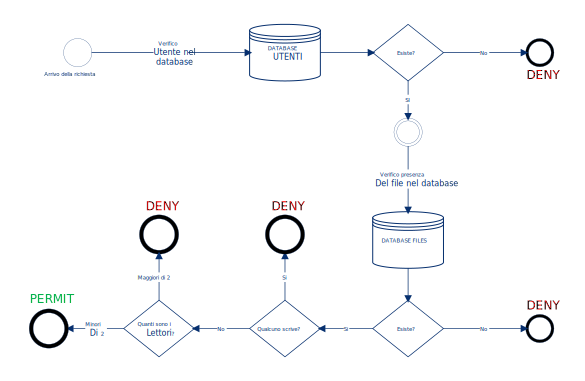
\includegraphics[scale = 0.75, , trim=1.5cm 0 0 0]{./Visio_Project/DiagrammaFlussoPrimoEsempio.pdf}
 \caption{Diagramma di flusso del primo esempio}
 \label{fig:diagrammaflussoprimoesempio}
\end{figure}

\subsection*{Esempio 2: Acquisto e noleggio di contenuti}
Un altro utilizzo possibile di \textit{Usage Control} riguarda l'analisi del comportamento passato. Un'azienda fornisce  ai propri clienti 
la possibilità di effettuare noleggi o acquisti di contenuti multimediali (musica, video, film, serie tv e via discorrendo).\\ \par
In caso il contenuto fosse stato acquistato, l’acquirente potrà ottenere
l’accesso infinite volte per infinito tempo. Nel caso di noleggio invece
saranno presenti delle condizioni, come per esempio il massimo numero
di fruizioni del contenuto o una data di scadenza che, una volta oltrepassata,
impedirà l’ulteriore visione del contenuto noleggiato in precedenza.
Come nell’esempio precedente viene proposto un diagramma di flusso,
proposto Figura~\ref{fig:diagrammaflussosecondoesempio}, che permette di capire meglio il funzionamento questo sistema di \textit{Usage Control}
\begin{figure}[H]
 \centering 
	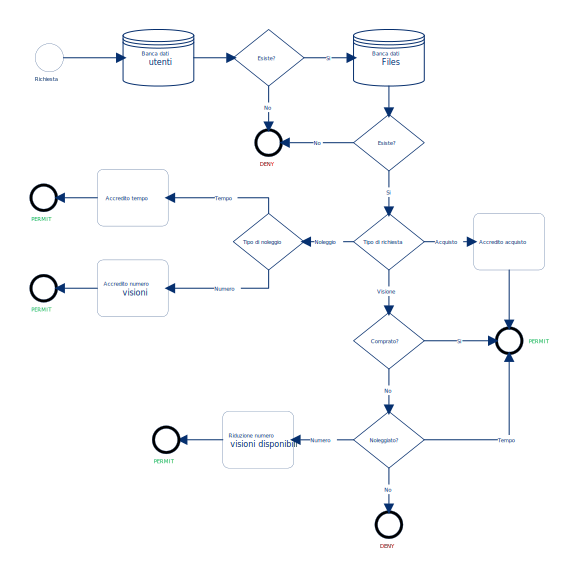
\includegraphics[scale = 0.75]{./Visio_Project/DiagrammaFlussoSecondoEsempio.pdf}
 \caption{Diagramma di flusso del secondo esempio}
 \label{fig:diagrammaflussosecondoesempio}
\end{figure}
